%!TEX root = ../main.tex
\documentclass[float=false, crop=false]{standalone}
\usepackage[subpreambles=true]{standalone}
\begin{document}
\section{Image test}\label{sec:imagetest}
In this section we will test the figure and subfigure environments. Placing figures is always as random as playing roulette in Vegas, double reds!
\subsection{Figures}
First we are testing a simple \texttt{JPEG} image in a single figure import:
\begin{figure}[h!]
    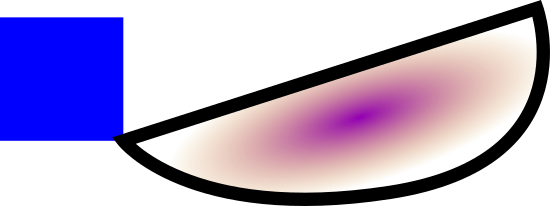
\includegraphics[width=\textwidth]{./img/rect10.png}
    \caption{Testing PDF image}
    \label{fig:pdftest}
\end{figure}
\subsection{Subfigures}
Now for adding subfigures.
\begin{figure}
    \centering
    \begin{subfigure}[h!]{0.5\linewidth}
        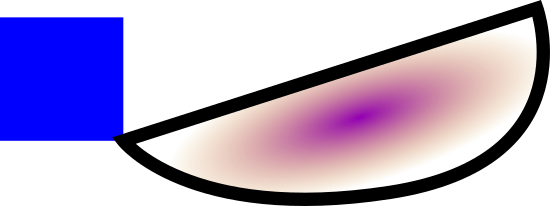
\includegraphics[width=\textwidth]{./img/rect10.png}
        \caption{Testing PDF image}
        \label{fig:pdftest}
    \end{subfigure}
    %add desired spacing between images, e. g. ~, \quad, \qquad, \hfill etc. 
      %(or a blank line to force the subfigure onto a new line)
    \begin{subfigure}[h!]{0.49\linewidth}
        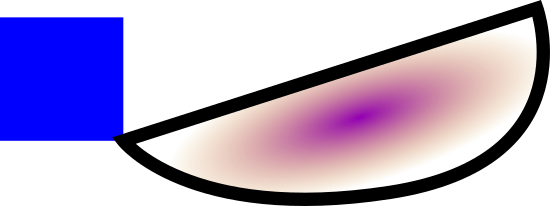
\includegraphics[width=\textwidth]{./img/rect10.png}
        \caption{Testing PNG}
        \label{fig:pngtest}
    \end{subfigure}
    ~ %add desired spacing between images, e. g. ~, \quad, \qquad, \hfill etc. 
      %(or a blank line to force the subfigure onto a new line)
    \caption{Testing subfigues image}
    \label{fig:pdftest}
\end{figure}
\end{document}